%---------------------------------------------------------------------------------------------------
\subsection{True Triaxial Test on the Cubic Opalinus Claystone Samples}
\label{sec:True_Triaxial_Exp}
\Authors{Amir Shoarian Sattari (CAU)}
%\todo{Please insert authors}

The true triaxial apparatus, where the stresses are controlled along three axes, is used to investigate the three-dimensional strain-strength behavior of soil or rock geomaterial (Figure \ref{fig:Amir_TrueTriaxial_Apparatus}). The true triaxial device in the CAU Kiel laboratory is able to reach a mechanical loading of 600 $MPa$ as well as a thermal loading of up to 600 $^{\circ}C$. The cubic samples are prepared in the side dimension of 43 $mm$ and the edges are slightly curved in order to avoid the stress concentration and failure in the corners (Figure \ref{fig:Amir_TrueTriaxial_Sample}).

\begin{figure}[!ht]
\begin{subfigure}[c]{0.48\textwidth}
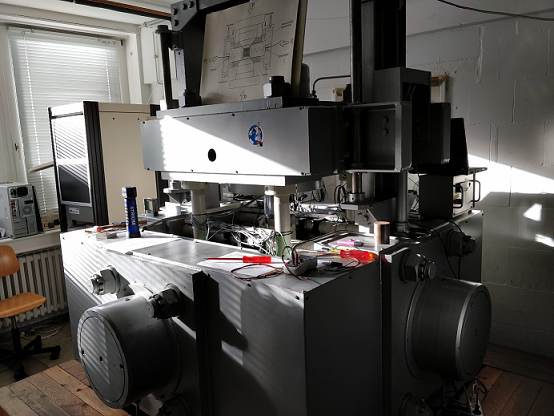
\includegraphics[width=1\textwidth]{figures/Amir_TrueTriaxial_Apparatus.png}
\subcaption{}
\label{fig:Amir_TrueTriaxial_Apparatus}
\end{subfigure}
\hfill
\begin{subfigure}[c]{0.48\textwidth}
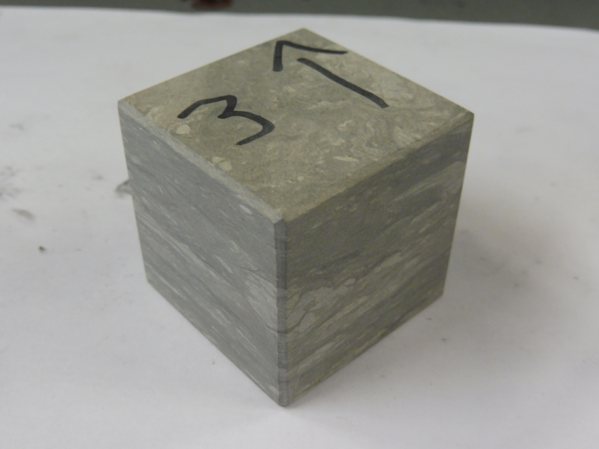
\includegraphics[width=1\textwidth]{figures/Amir_TrueTriaxial_Sample.png}
\subcaption{}
\label{fig:Amir_TrueTriaxial_Sample}
\end{subfigure}
\caption{The (a) true triaxial apparatus in geomechanics laboratory of CAU Kiel, and (b) prepared cubic claystone sample with curved edges}
\end{figure}

The coupled thermo-mechanical loading conditions are considered in order to investigate the materials anisotropic stiffness along three axis, the elastic and plastic deformation under cyclic thermal and mechanical loadings, deviatoric stress field, and material failure. A thermal loading of up to $T_{iso}^{max}=150$ $^{\circ}C$ is considered, which is considered to be higher than the maximum temperature that the claystone samples are subjected to in nuclear waste disposal sites. The maximum isotropic mechanical loading is considered to be $\sigma_{iso}^{max}=100 MPa$, where $max$ and $c$ superscripts represent the maximum and constant values, respectively. The considered boundary conditions are:

\begin{list}{-}{\leftmargin=1em \itemindent=0em \itemsep=0.1em}
  \item Sample MT-01: Mechanical Condition,5 loading cycles, $\sigma_{iso}^{max}=100 MPa$.
  \item Sample MT-02: Coupled Thermo-Mechanical Condition, 4 loading cycles, $T_{iso}^{max}=150$ $^{\circ}C$ and $\sigma_{iso}^{c}=12 MPa$.
  \item Sample MT-03: Coupled Thermo-Mechanical Condition, 4 loading cycles, $T_{iso}^{max}=150$ $^{\circ}C$, and $\sigma_{iso}^{max}=100 MPa$.
  \item Sample MT-04: Coupled Thermo-Mechanical Condition, 4 loading cycles, $\sigma_{dev}^{max}=60 MPa$, $\sigma_{con}^{c}= 20 MPa$ and $T_{iso}^{c}=150$ $^{\circ}C$ .
\end{list}

With the installation of the ultrasonic sensors on the pistons, the apparatus is able to measure the ultrasonic $P$, $S90$ and $S0$ waves along the axis. The anisotropy factor, density ($\rho$), the dynamic Young’s modulus ($E_{Dyn}$), dynamic shear modulus ($G_{Dyn}$), and dynamic Poisson’s ratio ($\nu_{Dyn}$) values can all be calculated according to the analytical relation which already exist in the literature \cite{Motraetal2018} as given in equations (\ref{eq:YoungsModulus_Ultrasonic}) and (\ref{eq:PoissonsRatio_Ultrasonic}). In order to detect and analyse the ultrasonic signals in Opalinus Claystone, the minimum confining mechanical stresses of 12 $MPa$ is required. The test results of MT-01 (Figure \ref{fig:Amir_TrueTriaxial_MT_01_Result}) depicts the increment of the mean $E_{Dyn}$, $G_{Dyn}$ and $\nu_{Dyn}$ values under the isotopic confinement stresses up to 100 $MPa$, which is due to the layering orientation and structure of claystones and eventually improved contact qualities. It is also noted that the rate of the increment after each loading cycle (slope of the line) is decreased and due to the plastic deformations and improved contact qualities, the materials mechanical properties in initial loading condition of 12 $MPa$ are enhanced. 

\begin{figure}[ht!]
\centering
\begin{subfigure}[c]{0.48\textwidth}
\centering
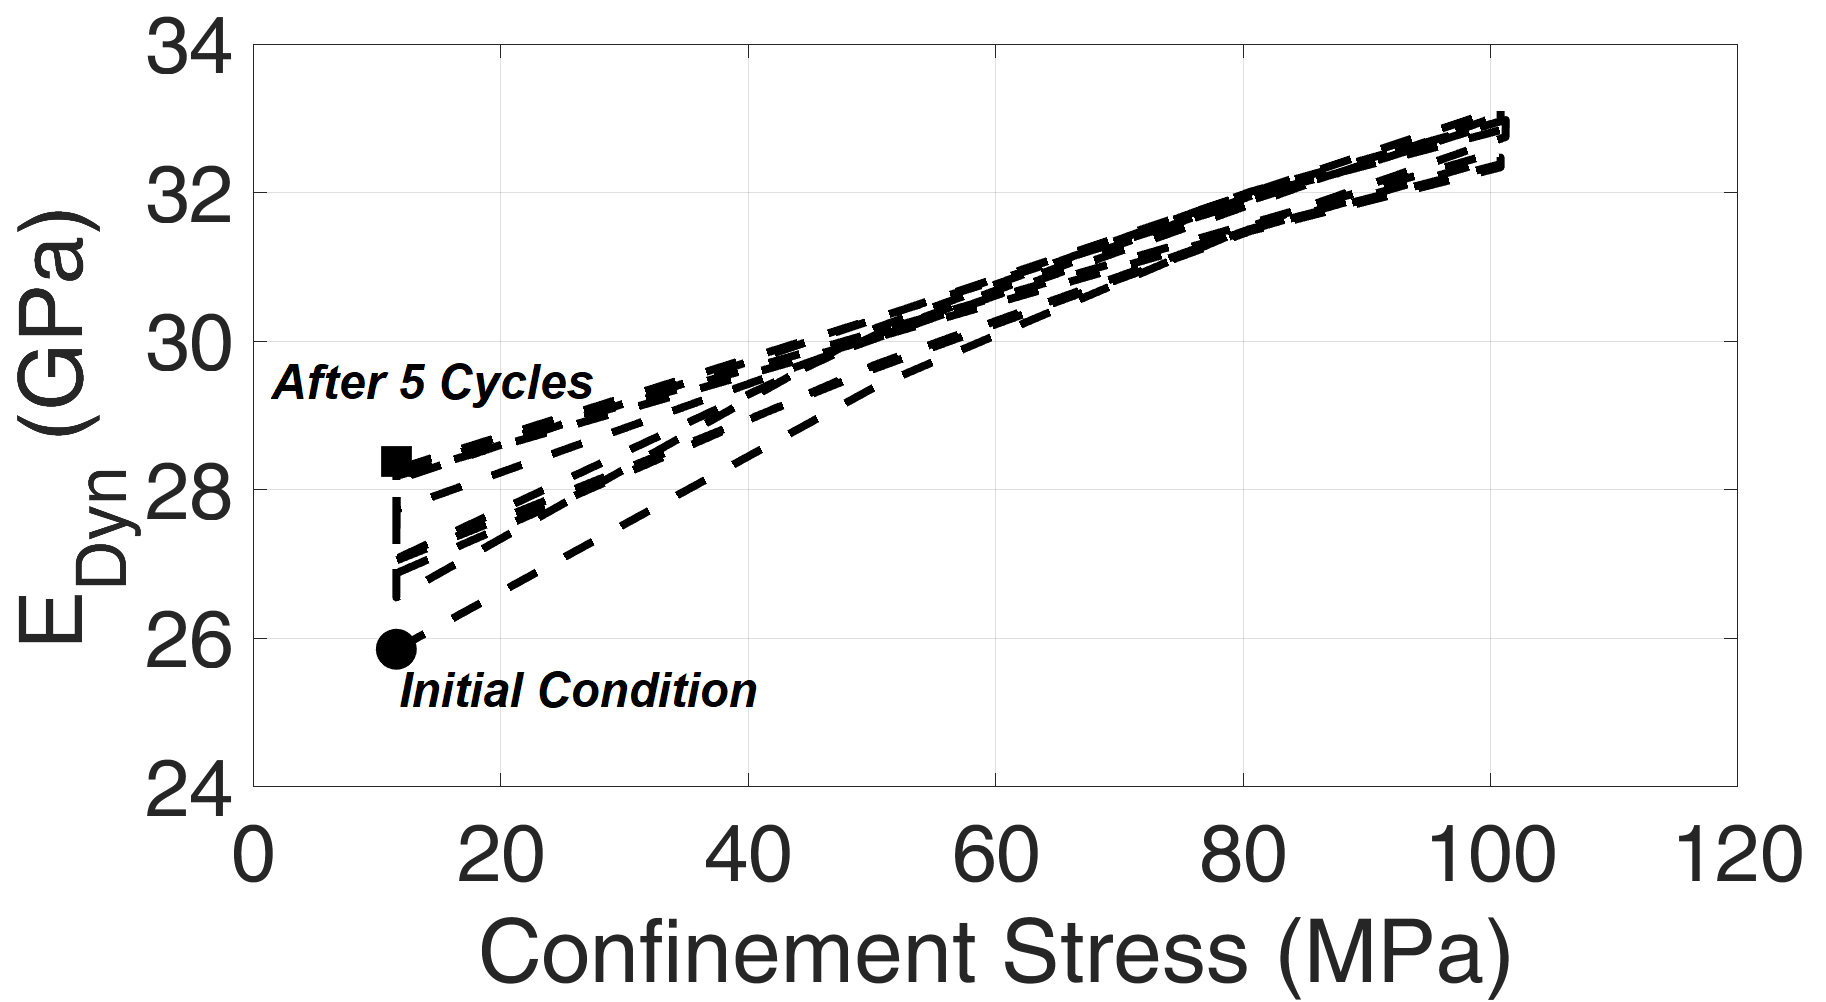
\includegraphics[width=6cm,height=4cm]{figures/Amir_TrueTriaxial_MT_01_Result_E.png}
\subcaption{}
\end{subfigure}
\hfill
\begin{subfigure}[c]{0.48\textwidth}
\centering
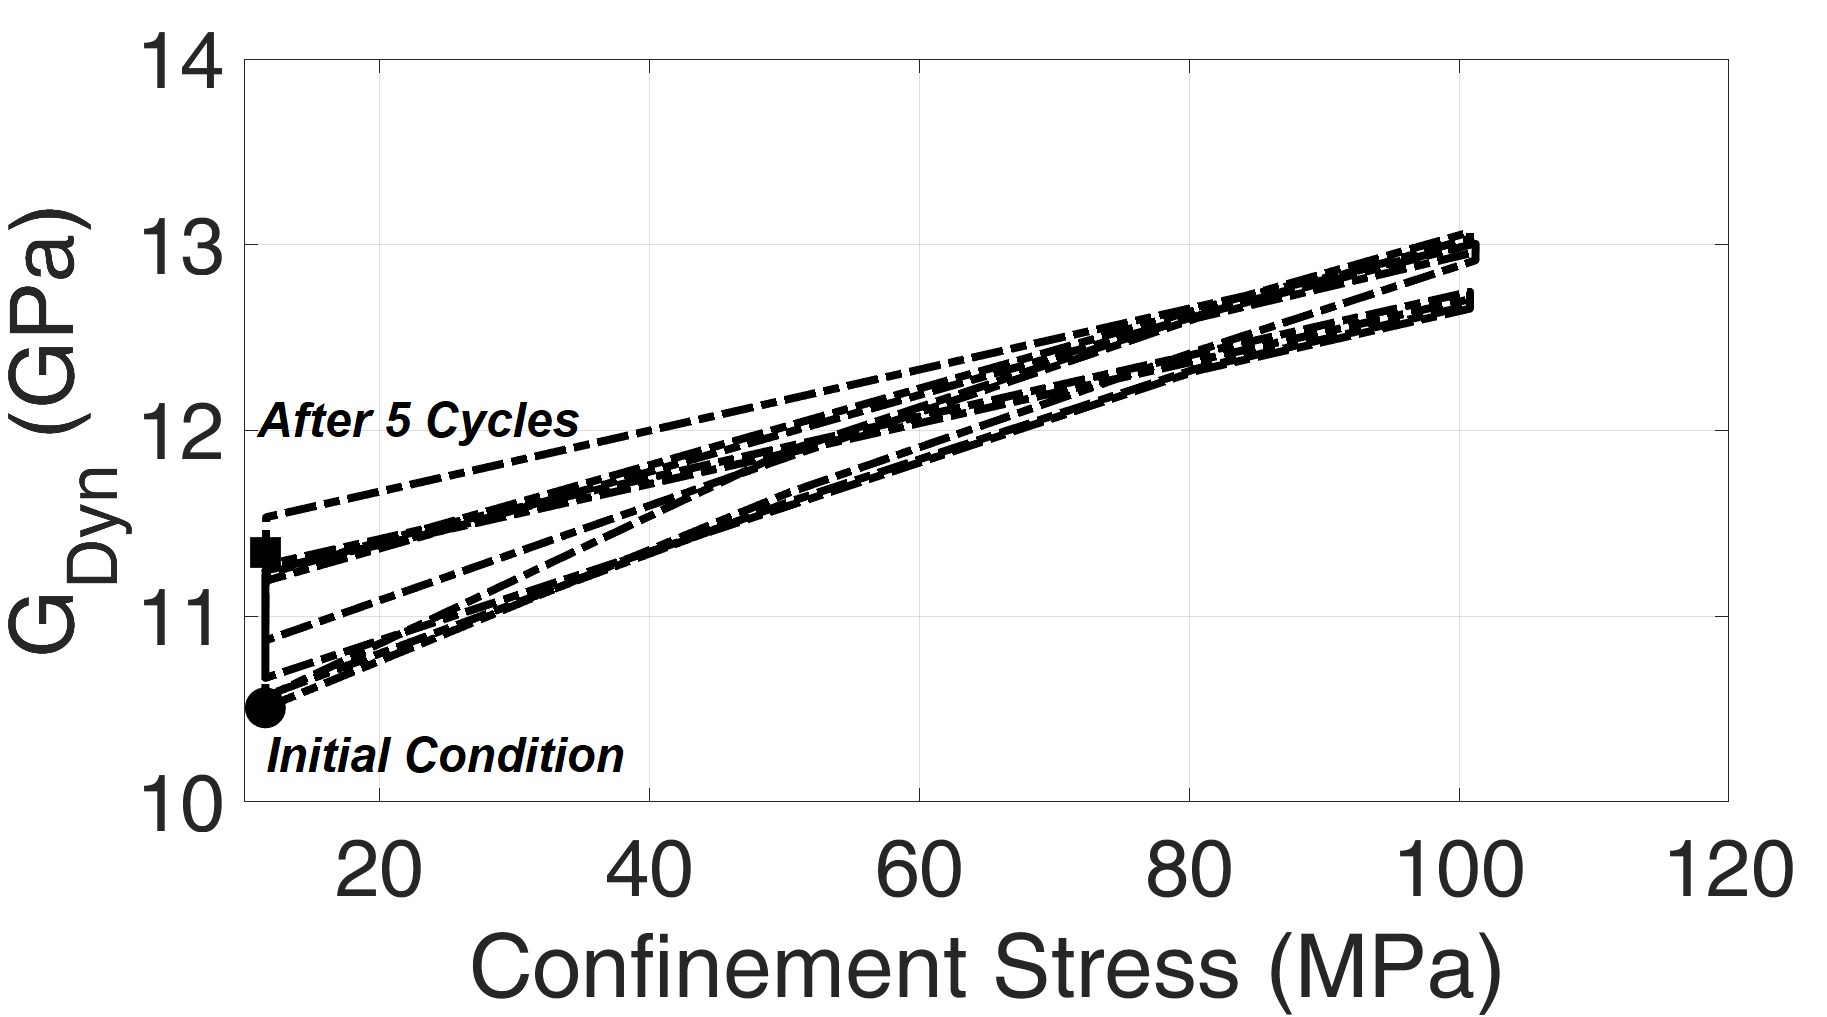
\includegraphics[width=6cm,height=4cm]{figures/Amir_TrueTriaxial_MT_01_Result_G.png}
\subcaption{}
\end{subfigure}
\hfill
\begin{subfigure}[c]{0.48\textwidth}
\centering
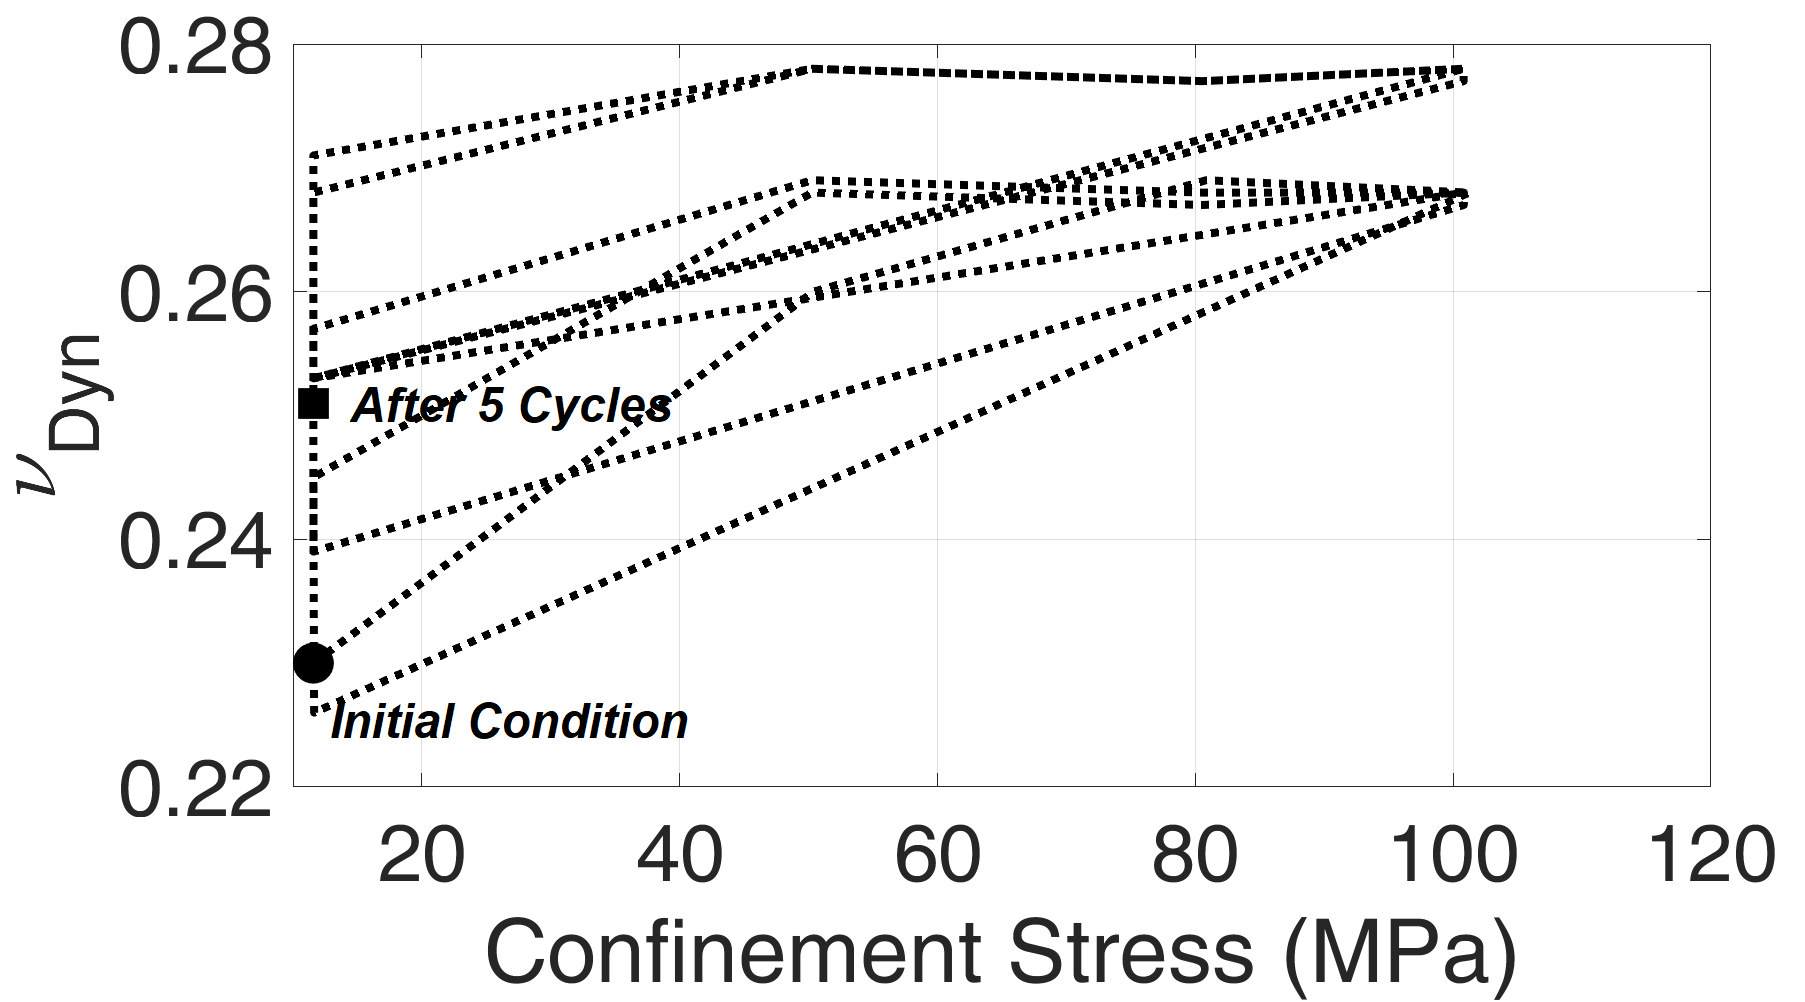
\includegraphics[width=6cm,height=4cm]{figures/Amir_TrueTriaxial_MT_01_Result_Nu.png}
\subcaption{}
\end{subfigure}
\caption{The true triaxial results for the MT-01 sample under 5 loading cycles (a) $E_{Dyn}$ vs. Confinement Stress, (b) $G_{Dyn}$ vs. Confinement Stress, and (c) $\nu_{Dyn}$ vs. Confinement Stress}
\label{fig:Amir_TrueTriaxial_MT_01_Result}
\end{figure}

Figure \ref{fig:Amir_TrueTriaxial_MT_02_Result} shows the deformation vs. time result of MT-02 in the 1st cycle. The thermal plastic deformation after 5 cycles of loading and unloading was negligible and can be neglected. The MT-02 sample is situated in a way that the loading frame in direction of Z is parallel to the layering orientations of claystone. The volumetric thermal expansion coefficient ($\alpha_V$) is calculated based on the measured volumetric strain ($\epsilon_V=\frac{\Delta V}{V}$) and temperature change ($\Delta T$). The effect of temperature on $\alpha_V$ is shown at Figure \ref{fig:Amir_TrueTriaxial_MT_02_Result_1a}. The rate of $\alpha_V$ is decreased after 80 $^{\circ}C$. The anisotropy in linear thermal expansion coefficient along Z, Y and X axis is shown in Figure \ref{fig:Amir_TrueTriaxial_MT_02_Result_1b}. The anisotropy in the measured linear expansion coefficient ($\alpha_{Li}$) is substantially decreased after 80 $^{\circ}C$.

\begin{align}
\label{eq:ThermalExpansion}
\begin{split}
\alpha_V=\frac{\epsilon_V}{\Delta T}=\frac{\Delta V}{V\Delta T}
\end{split}
\end{align}

\begin{figure}[!ht]
\centering
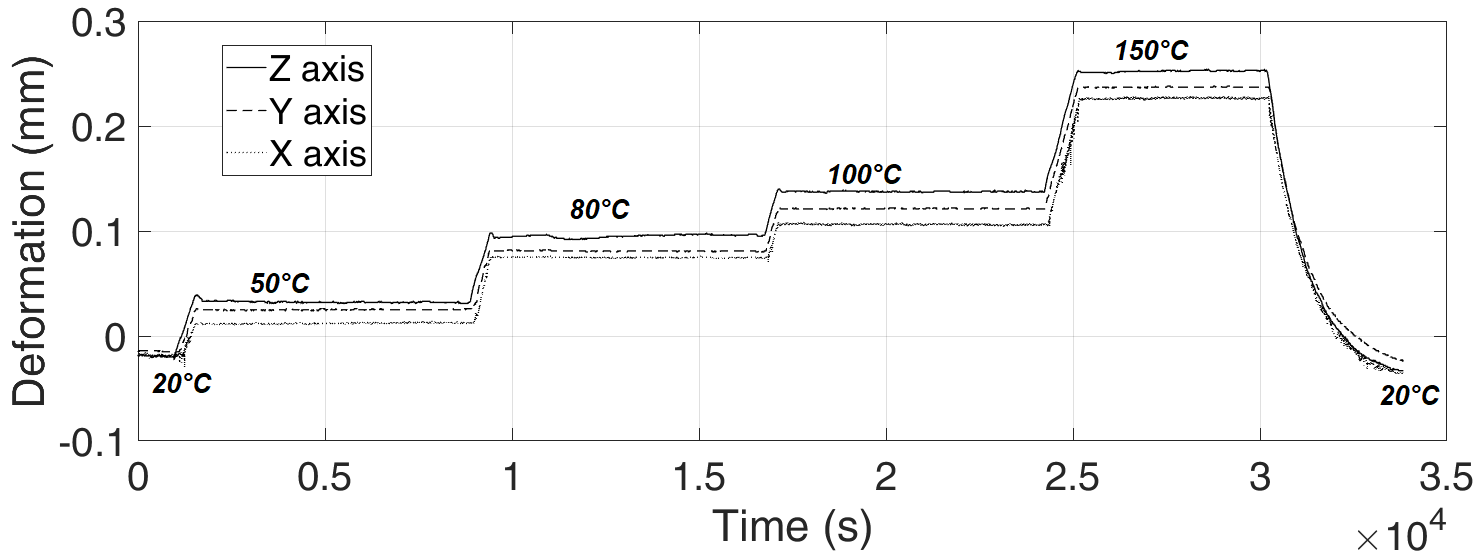
\includegraphics[width=7cm,height=4cm]{figures/Amir_TrueTriaxial_MT_02_Result.png}
\caption{The deformation vs time for sample MT-02}
\label{fig:Amir_TrueTriaxial_MT_02_Result}
\end{figure} 

\begin{figure}[!ht]
\centering
\begin{subfigure}[c]{0.48\textwidth}
\centering
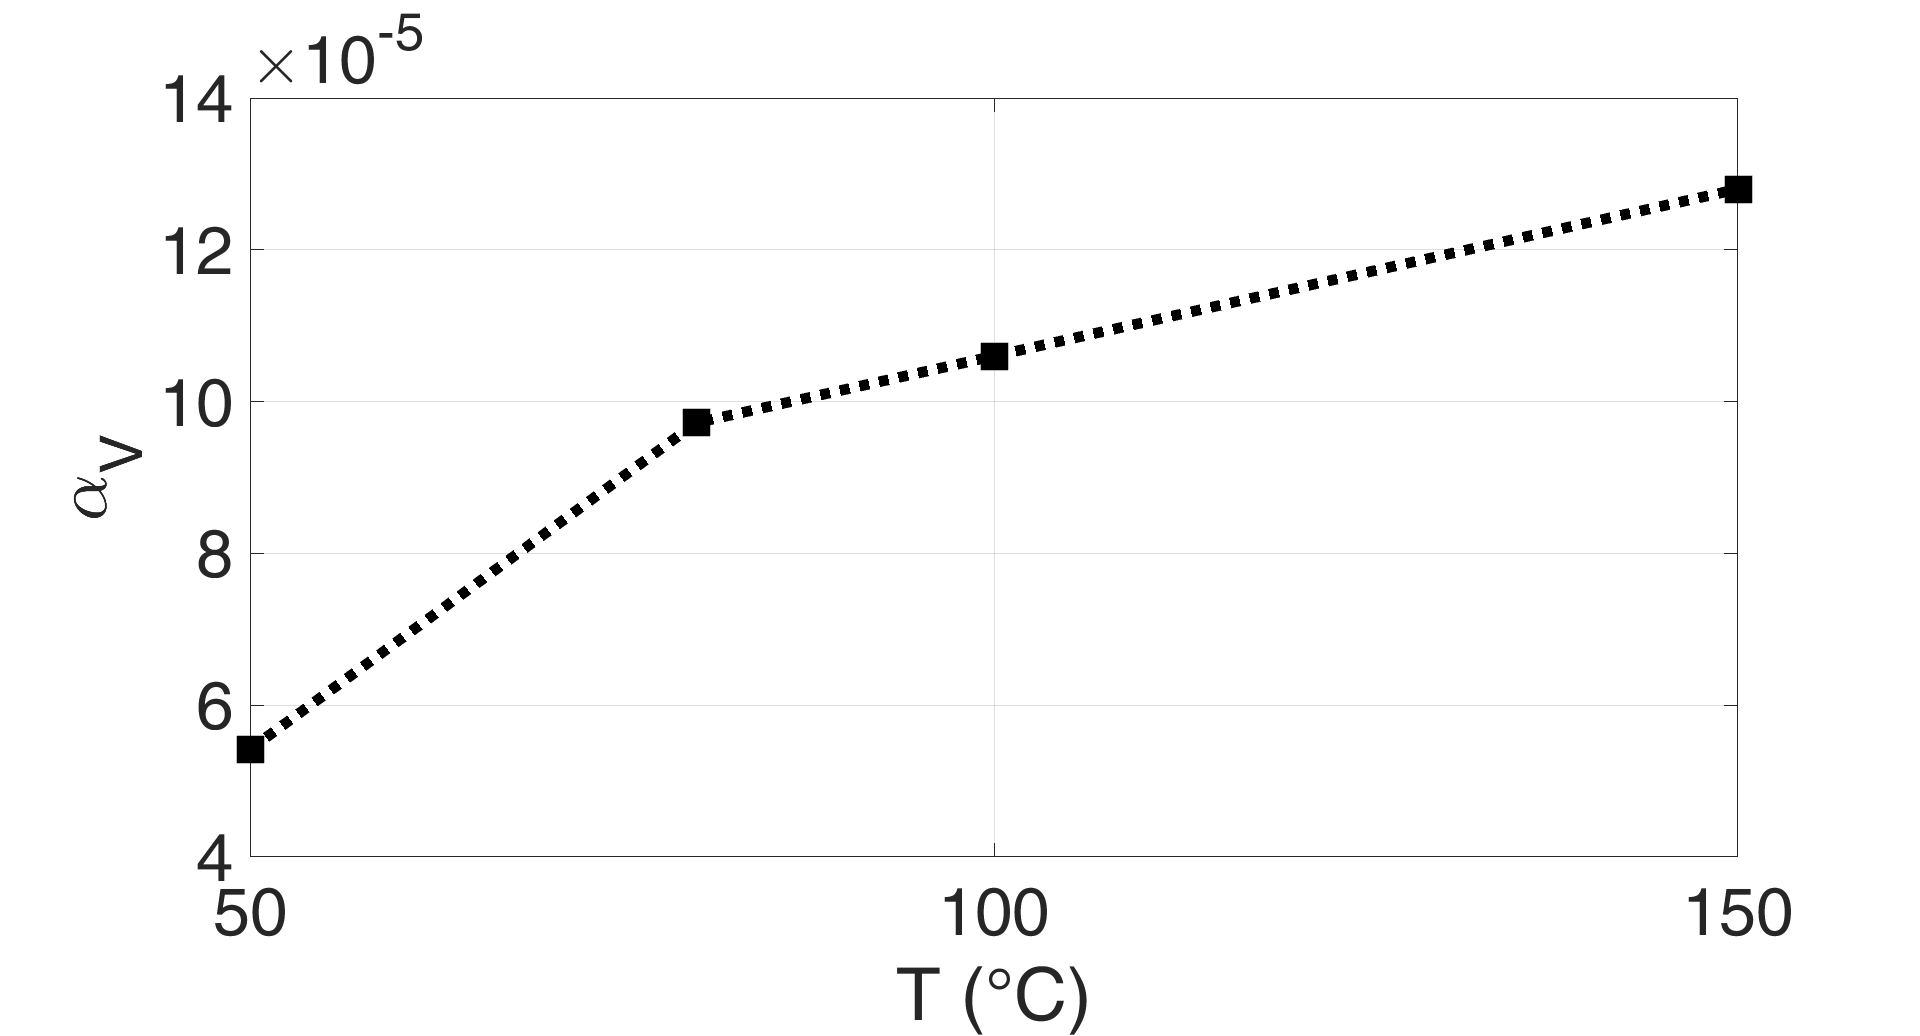
\includegraphics[width=6cm,height=4cm]{figures/Amir_TrueTriaxial_MT_02_Result_1a.png}
\subcaption{}
\label{fig:Amir_TrueTriaxial_MT_02_Result_1a}
\end{subfigure}
\hfill
\begin{subfigure}[c]{0.48\textwidth}
\centering
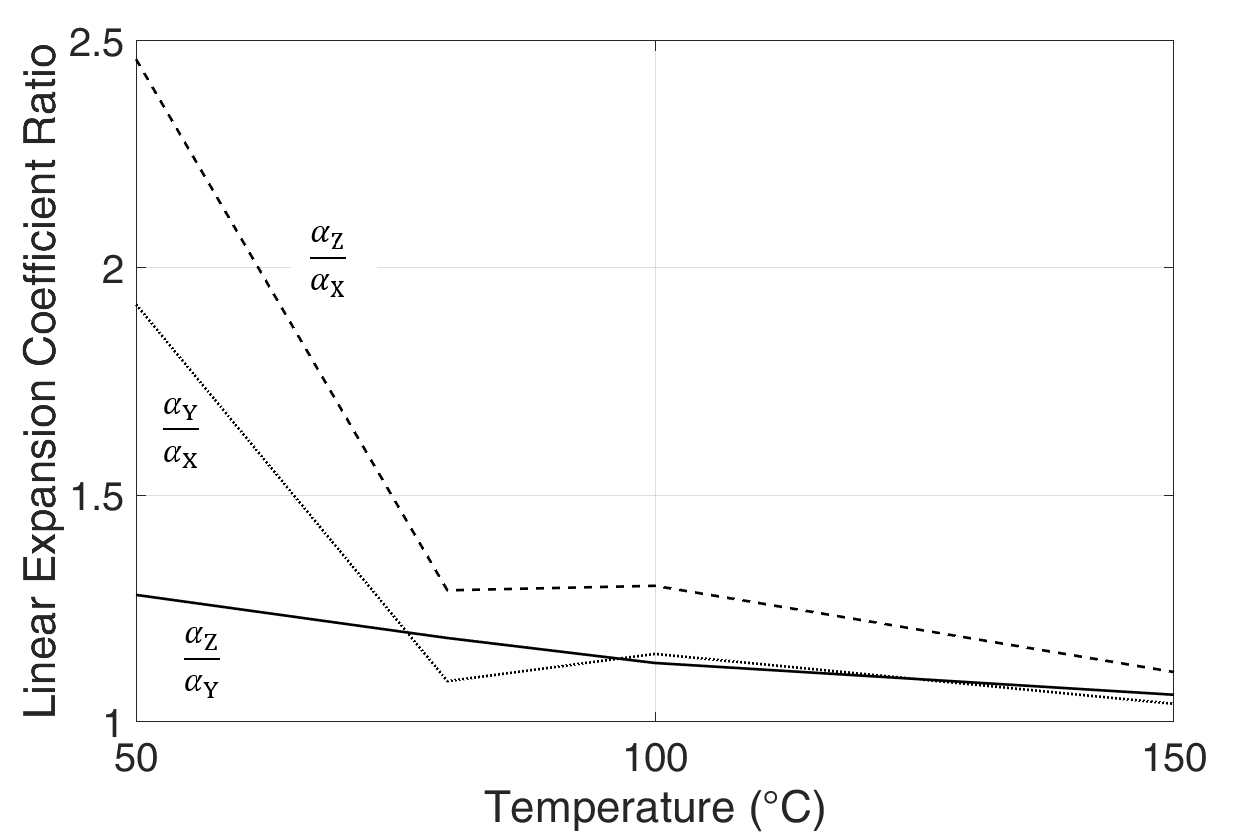
\includegraphics[width=6cm,height=4cm]{figures/Amir_TrueTriaxial_MT_02_Result_1b.png}
\subcaption{}
\label{fig:Amir_TrueTriaxial_MT_02_Result_1b}
\end{subfigure}
\caption{The effect of temperature on (a) $\alpha_V$, and (b) the anisotropy in the linear thermal expansion coefficient ($\alpha_{Li}$)}
\end{figure}

The test results of MT-03 investigates the anisotropy of Opalinus claystone samples. Figure \ref{fig:Amir_TrueTriaxial_MT_03_Result} illustrates the $1^{st}$ cycle loading results of $E_{Dyn}$ and $\nu_{Dyn}$ values in X, Y and Z directions under the isotopic confinement stresses up to 100 $MPa$. The $G_{Dyn}$ has a similar behavior to the $E_{Dyn}$ values. The results indicate a weaker stiffness in Z direction, which is parallel to the layering orientation. The thermal loading upto 150 $^{\circ}C$ results in weaker $E_{Dyn}$ values during the heating process, which is the reason for the fluctuation of the results at the confinement stress of 100 $MPa$. The test results of MT-04 is similar to the MT-02 and the same material response is observed. 

\begin{figure}[ht!]
\centering
\begin{subfigure}[c]{0.48\textwidth}
\centering
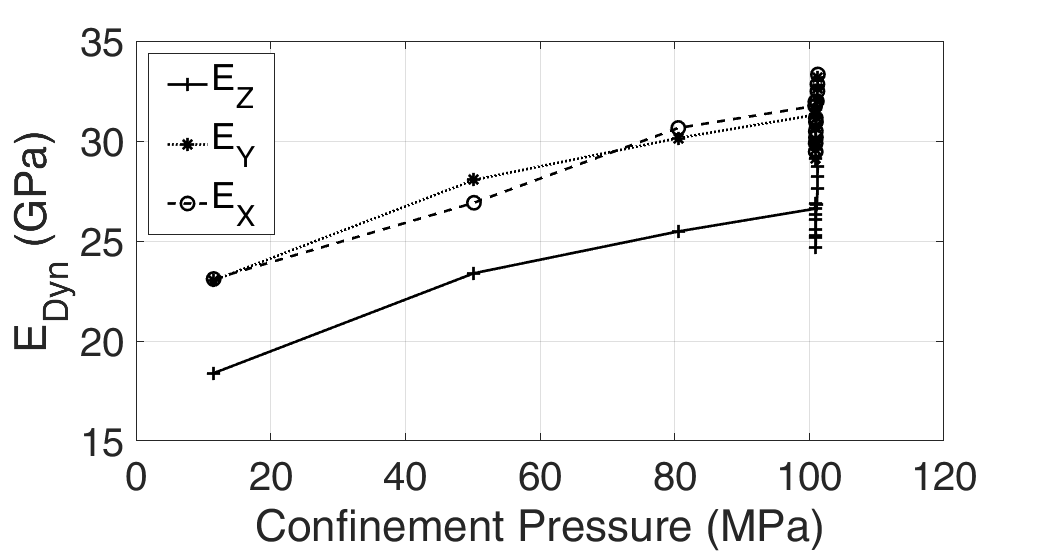
\includegraphics[width=6cm,height=4cm]{figures/Amir_TrueTriaxial_MT_03_Result_E.png}
\subcaption{}
\end{subfigure}
\hfill
\begin{subfigure}[c]{0.48\textwidth}
\centering
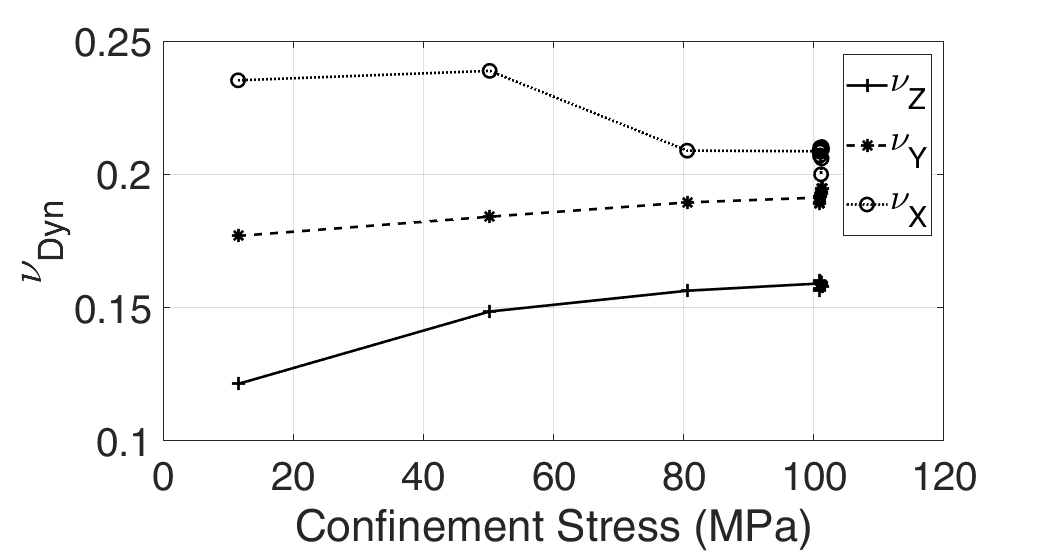
\includegraphics[width=6cm,height=4cm]{figures/Amir_TrueTriaxial_MT_03_Result_Nu.png}
\subcaption{}
\end{subfigure}
\caption{The true triaxial results for the MT-03 sample in the $1^{st}$ cycle (a) $E_{Dyn}$ vs. Confinement Stress, and (b) $\nu_{Dyn}$ vs. Confinement Stress}
\label{fig:Amir_TrueTriaxial_MT_03_Result}
\end{figure}